\documentclass[
	classe=$2^{de}$
]{coursclass}

\usetikzlibrary{calc}

\renewcommand{\arraystretch}{1.5}

\title{Chapitre 8 : Probabilités}
\author{}
\date{}

\begin{document}

\maketitle

\begin{definition}[Univers, issues, évènements]
	\begin{itemize}
		\item Une \textbf{expérience aléatoire} est une expérience dont on ne peut pas prédire le résultat à l'avance.
		\item Lorsqu'on fait une expérience aléatoire, les résultats que l'on peut obtenir sont appelés les \textbf{issues}.
		\item L'ensemble complet des issues est appelé \textbf{l'univers}. On le note généralement $Ω$.
		\item Un ensemble d'issues est un \textbf{évènement}. On le note généralement avec une lettre majuscule, comme $A$, $B$, ...
		\item Si on a un évènement $A$, on appelle $\overline{A}$ l'\textbf{évènement contraire} de $A$ : c'est l'évènement qui contient les issues qui ne sont pas dans $A$.
	\end{itemize}
\end{definition}

\begin{exemple}
	\begin{itemize}
		\item Si on lance un dé et qu'on regarde le résultat, il s'agit d'une expérience aléatoire.
		\item Les issues sont alors $1$, $2$, $3$, $4$, $5$ et $6$. L'univers est $Ω = \{1, 2, 3, 4, 5, 6\}$.
		\item On peut noter $A$ l'évènement « Le résultat obtenu est pair ». $A$ contient alors les issues $2$, $4$ et $6$.
		\item $\overline{A}$ contient les issues $1$, $3$ et $5$.
	\end{itemize}
\end{exemple}

\begin{definition}[Loi de probabilité]
	Si on a un univers, une \textbf{loi de probabilité} consiste à :
	\begin{itemize}
		\item Associer un probabilité entre $0$ et $1$ à chaque issue ;
		\item Tel que la somme des probabilités des issues soit $1$.
	\end{itemize}
\end{definition}

\begin{exemple}
	\begin{multicols}{2}
		La loi de probabilité d'un dé est :
		\begin{center}
			\begin{tabular}{|l|c|c|c|c|c|c|}
				\hline
				Issue       & $1$           & $2$           & $3$           & $4$           & $5$           & $6$           \\ \hline
				Probabilité & $\frac{1}{6}$ & $\frac{1}{6}$ & $\frac{1}{6}$ & $\frac{1}{6}$ & $\frac{1}{6}$ & $\frac{1}{6}$ \\ \hline
			\end{tabular}
		\end{center}

		\columnbreak

		La loi de probabilité d'un dé truqué peut être :
		\begin{center}
			\begin{tabular}{|l|c|c|c|c|c|c|}
				\hline
				Issue       & $1$           & $2$           & $3$           & $4$           & $5$           & $6$           \\ \hline
				Probabilité & $\frac{1}{12}$ & $\frac{1}{3}$ & $\frac{1}{12}$ & $\frac{1}{4}$ & $\frac{1}{6}$ & $\frac{1}{12}$ \\ \hline
			\end{tabular}
		\end{center}
	\end{multicols}
\end{exemple}

\begin{definition}[Arbre de probabilités]
	Une expérience aléatoire peut être représentée par un \textbf{arbre de probabilités} si elle est composée de plusieurs \textbf{épreuves} qui se suivent.
\end{definition}

\begin{exemple}
	\begin{minipage}{0.4\linewidth}
		On fait une expérience qui consiste à :
		\begin{itemize}
			\item Lancer une pièce à pile ou face
			\item Lancer un dé équilibré, et regarder si on a fait un $6$.
		\end{itemize}
	\end{minipage}
	\begin{minipage}{0.55\linewidth}
		\begin{center}
			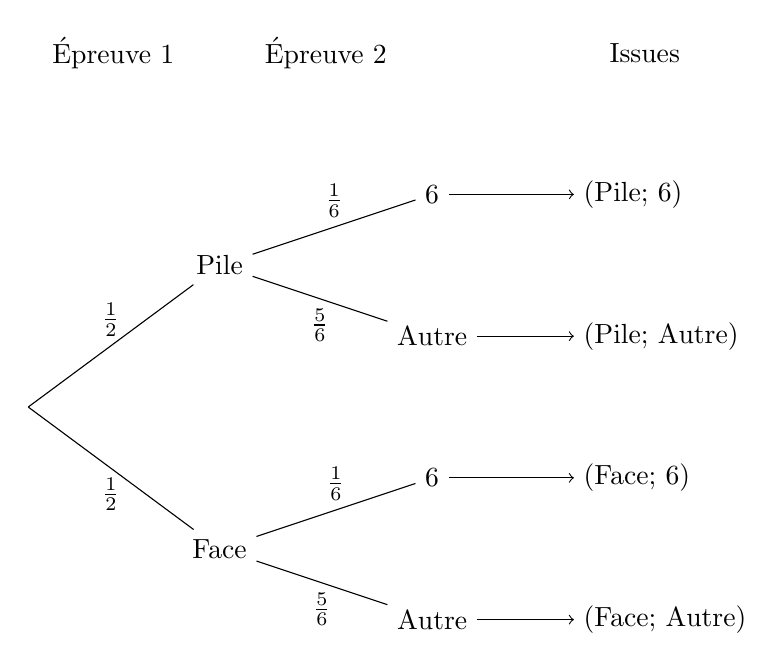
\begin{tikzpicture}[scale=0.9]
				\coordinate (START) at (0.3,0);

				\node at (1.5,5) {Épreuve 1};
				\node at (4.5,5) {Épreuve 2};
				\node at (9,5) {Issues};

				\node (Pile) at (3,2) {Pile};
				\node (Face) at (3,-2) {Face};
				\draw (START) -- node[above] {$\frac{1}{2}$} (Pile)
				(START) -- node[below] {$\frac{1}{2}$} (Face);
				\foreach \n in {Pile,Face} {
						\node (Ab) at ($(\n) + (3,1)$) {$6$};
						\node (NAb) at ($(\n) + (3,-1)$) {Autre};
						\draw (\n) -- node[above] {$\frac{1}{6}$} (Ab);
						\draw (\n) -- node[below] {$\frac{5}{6}$} (NAb);

						\draw[->] (Ab) -- ++(2,0) node[right] {(\n ; $6$)};
						\draw[->] (NAb) -- ++(2,0) node[right] {(\n ; Autre)};
					}
			\end{tikzpicture}
		\end{center}
	\end{minipage}
\end{exemple}

\begin{propriete}
	Pour obtenir la probabilité d'une issue, on \textbf{multiplie} les probabilités sur les branches menant à cette issue.
\end{propriete}

\begin{exemple}
	Sur l'exemple ci-dessus les probabilités sont :
	\begin{itemize}
		\item (Pile ; $6$) → $\dfrac{1}{2} × \dfrac{1}{6} = \dfrac{1}{12}$
		\item (Pile ; Autre) → $\dfrac{1}{2} × \dfrac{5}{6} = \dfrac{5}{12}$
		\item (Face ; $6$) → $\dfrac{1}{2} × \dfrac{1}{6} = \dfrac{1}{12}$
		\item (Face ; Autre) → $\dfrac{1}{2} × \dfrac{5}{6} = \dfrac{5}{12}$
	\end{itemize}
\end{exemple}

\begin{propriete}
	Pour obtenir la probabilité d'un évènement, on \textbf{additionne} les probabilités des issues qui le constitue.
\end{propriete}

\begin{exemple}
	Si on cherche la probabilité de l'évènement «On a fait face OU on a fait un $6$», les issues \ (Pile ; $6$), (Face ; $6$) ou (Face ; Autre) conviennent.

	La probabilité de cet évènement est donc $\dfrac{1}{12} + \dfrac{1}{12} + \dfrac{5}{12} = \dfrac{7}{12}$.
\end{exemple}

\end{document}